\chapter{Dataset}
\label{chap:dataset}

Datasets are important part of every research project\ms{s}, you can either use it to evaluate your models or even train your models. Then the gold mind is every labelled dataset which provides the ground truth. The problem is that each dataset is really field specific so in our case we cannot use, for instance, a dataset of handwritten digits for our case. Another problem with the kind of data we need is that it can be really big. \cite{xu2009detecting} worked with Hadoop cluster logs generated in range of 48 hours by more than 200 nodes with total volume bigger than 200 TB, which were not, unfortunately, shared any further.

\section{Existing datasets}

Specific focus of this thesis limits us in what available dataset can be useful. The following list names the one we found:

\begin{itemize}

    \item \textbf{NAB\footnote{\url{https://github.com/numenta/NAB}}} - Numenta Anomaly Benchmark introduced in \cite{ahmad2017unsupervised} containes real-world and artificial time serias which can serve us for training time series monitoring based anomaly detection such we listed in \ms{Section}~\ref{ssec:sota_logging_monitoring}. Especially data for AWS cloud watch which covers CPU utilization, network traffic and Drive I/O and time series from section Known causes with misconfiguration causing CPU problems and system failure resulting EC2 request latency.
    
    \item \textbf{ODDS\footnote{\url{http://odds.cs.stonybrook.edu}}} - Outlier Detection DataSets collects multiple different datasets for outlier/anomaly detection since 2016 from all the interest fields around. Even though we did not find any dataset which would 100\% fit\ms{s} to our research it can be useful for general testing of state clarification of anomalies\ms{ under some assumptions I guess}. 
    
    \item \textbf{Loghub\footnote{\url{https://github.com/logpai/loghub}}} can provide a large collection of system logs per stand alone applications. This collection is cited and used by most of the recent papers and works dealing with system log parsing and analysing.

   \item \textbf{HDFS\footnote{\url{https://figshare.com/articles/HDFS_Logs/4040124}} \cite{xu2009detecting,xu2009online,Zhu2017}} contains log from more than 200 Hadoop nodes labelled by a Hadoop expert. There are about 2.9\% anomaly behaviour segments along more than 11 millions logged events total. This dataset was also used by many works we are refereeing in \ms{C}hapter~\ref{chap:stateOfTheArt}.
    
\end{itemize}

\section{Our new dataset}

Unfortunately, none of the datasets listed above fully represents a complex software architecture by our definition of complex software architecture \ms{(Definition~\ref{def:complexSoftwareArch})}. We had a chance to create such dataset in cooperation with SAP Concur and discuss it in this section.

\subsection{Service architecture}

SAP concur has a team which is responsible for internal 

\subsection{Problems}

\subsection{Current alerting system}

\subsection{Log structure}









\begin{figure}[h]
    \centering
    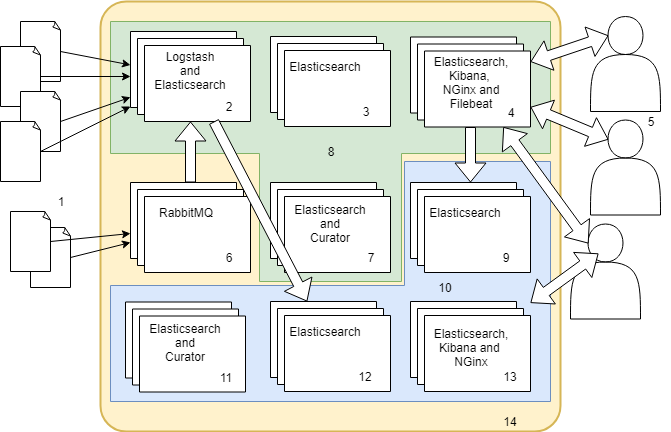
\includegraphics[width=0.9\textwidth]{figures/dataset/Parpr1Model.png}
    \caption[Illustration of a logging platform in one environment.]{Illustration of a logging platform in one environment. Explanatory notes: 1. incoming documents from users, 2. collector nodes with Logstash and Elasticsearch instance, 3. Elasticsearch data nodes of the green cluster, 4. servers running Kibana for log visualisation, 5. users, 6. RabbitMQ cluster, 7. Elasticsearch master nodes of the green cluster of the green cluster, 8. green cluster, 9. Elasticsearch ingests nodes, 10. blue cluster, 11. Elasticsearch master nodes of the blue cluster, 12. Elasticsearch data nodes of blue cluster, 13. servers running Kibana for log visualisation of the blue cluster, 14. logging platform environment setup}
    \label{fig:loggingPlatformIlustration}
\end{figure}